% !TEX root = ../thesis.tex
%
\chapter{Evaluation}
\label{sec:evaluation}

In this chapter performance characteristics of the implemented runtime and also of the instrumentation pass are presented.
To do so both systems are tested under a number of different circumstances to get an overview of how they might perform in real world usage.
As the complete benchmark data is to big in this chapter only summarys are presented.
The complete datasets can be found in \cref{sec:appendix}.

\section{Runtime Benchmarks}
\label{sec:evaluation:runtime_benchmarks}

Over the course of this thesis two different approaches to handling the progress of streams in the runtime are explored, which were also briefly mentioned in \cref{sec:definitions:run}: progress timestamps and progress events.
Progress timestamps were used first, which worked, but lead to big overhead when a great number of computations had to happen, since the whole stream had to be send to all children of the node that performed the computation.
Therefore, later the runtime was refactored to use progress events, so that only events had to be sent between nodes.
The following benchmarks will show the performance characteristics of both approaches under different circumstances.

\subsection{Number of Processors}
\label{sec:evaluation:runtime_benchmarks:num_cores}

Since one of the main motivations to choose Erlang as the plattform for the runtime was its support for parallel execution on many processor cores, we explore the performance characteristic in regard to available cores in this section.
To do so a simple \gls{tessla} specification is given, that includes as many nodes as the maximal number of processors available.
Such a spec for eigth processors is given in \cref{listing:runtime_parallel_spec_8}.

\begin{figure}
  \lstinputlisting[caption=\gls{tessla} specification with eight nodes on the critical path,label=listing:runtime_parallel_spec_8]{content/code/parallel_8.spec}
\end{figure}

The specification is evaluated over appropriate traces with a specified amount of processor cores available.
The needed time of the evaluation engine from its start until it emits the conclusion, that the stream \(\mathit{done}\) is \(\mathit{true}\), is measured for different amounts of processors.
All benchmarks were performed on the same machine  with upto 16 cores and 48GB of RAM.
\Cref{fig:chap_eval:runtime_num_cores} shows the results of the benchmarks.
The complete data can be found in \cref{table:tessla_server_v1_num_cores_data,table:tessla_server_v1_num_cores_data,table:tessla_server_v1_num_cores_data}.

\begin{figure}
  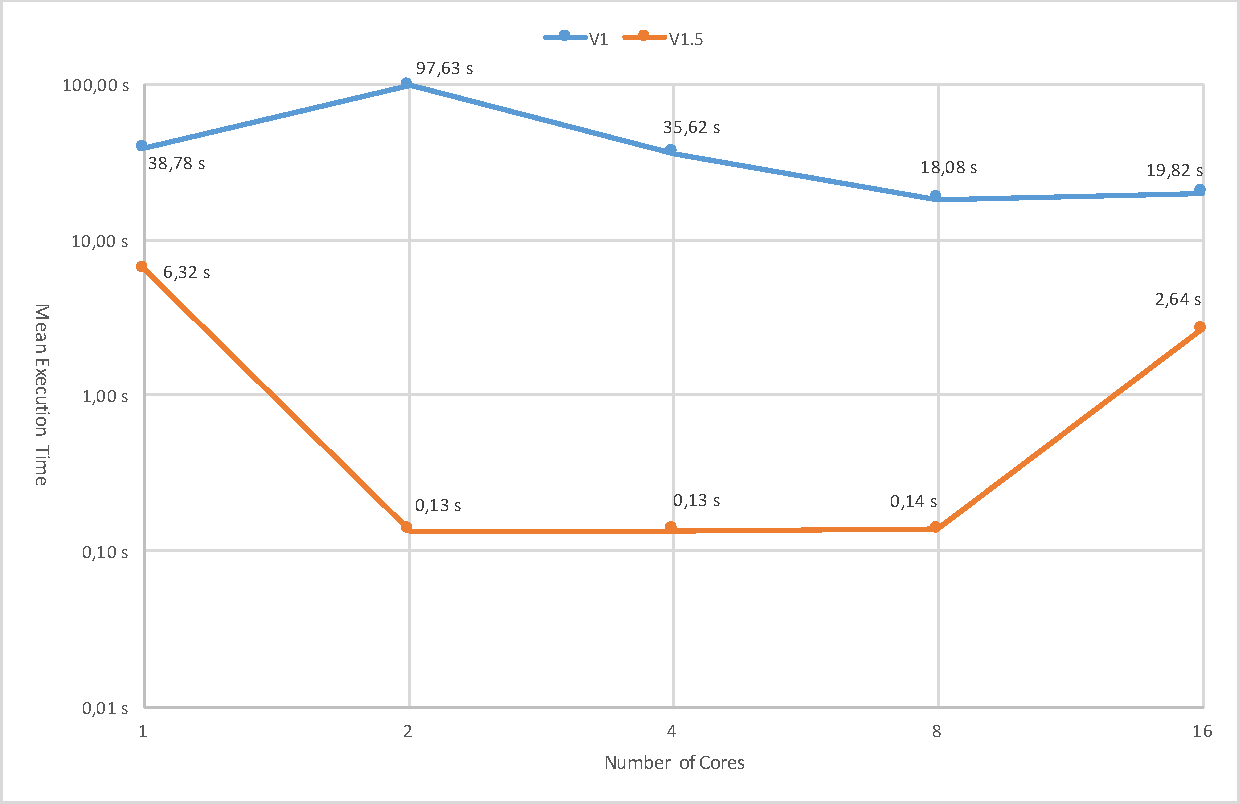
\includegraphics[width=\textwidth]{gfx/runtime_num_cores_benchmark}
  \caption[Performance of the runtime with different number of used cores]{Performance of the runtime with different number of used cores. V1 denotes the old implementation, V1.5 the adaption with limited amount of saved events and V2 the new approach.}
\label{fig:chap_eval:runtime_num_cores}
\end{figure}

One thing that was recognized during benchmarking was that the older implementation approach used big amounts of \gls{ram} and the usage grows exponentially with the amount of cores used .
For example, with two used cores the runtime would use around 2GB RAM, with 4 Cores already over 8GB.
This can be explained easily: in the old implementation all data has to be sent between all cores while in the new implementation only the generated events have to be sent around.
The excessive usage of \gls{ram} even lead to timeout under some circumstances and crashes the whole runtime.
The amount of data send between processes can even lead to negative performance impacts when more cores are added.

This behaviour was one of the main reasons to switch to a new approach.
To test if reduced \gls{ram} usage would lead to better performance and eliminate crashes, the old architecture was changed in a small way: Each stream was limited to only hold the last 20 events, all older events were thrown away.
Since the specification used for benchmarking only works on the most recent event of each stream, this would not alter the conclusion of the engine.
For example a specification computing the average of the last 21 events wouldn't work with this adaption.
See \cref{sec:evaluation:runtime_benchmarks:num_events} for a benchmark of \gls{ram} usage.
The obvious reduction of \gls{ram} usage of the adapted first approach motivated the decision to refactor the runtime to use the new approach.

TODO: describe how V2 scales with core number.

\subsection{Number of Events}
\label{sec:evaluation:runtime_benchmarks:num_events}

Another metric looked at, is how the runtime behaves in regard to the number of events that are fed to the engine, and therefore how many events are generated during its execution.
To obtain these metrics the specification from \cref{listing:runtime_parallel_spec_8} is evaluated with different values for the comparision node are run.
The specification is extended to use 16 nodes, which means that each input event will generate 16 internal events.
All benchmarks in this section were performed on a processor with 4 cores at 2.4GHz speed and 8GB of RAM.

The first benchmark compares the execution time of the implementation approaches when fed with different number of input events.
\Cref{fig:chap_eval:runtime_num_events} gives an overview of the data, the whole dataset can be found in \cref{table:tessla_server_v1_events_num_events_data,table:tessla_server_v1_5_events_num_events_data,table:tessla_server_v2_events_num_events_data}.

\begin{figure}[!htb]
  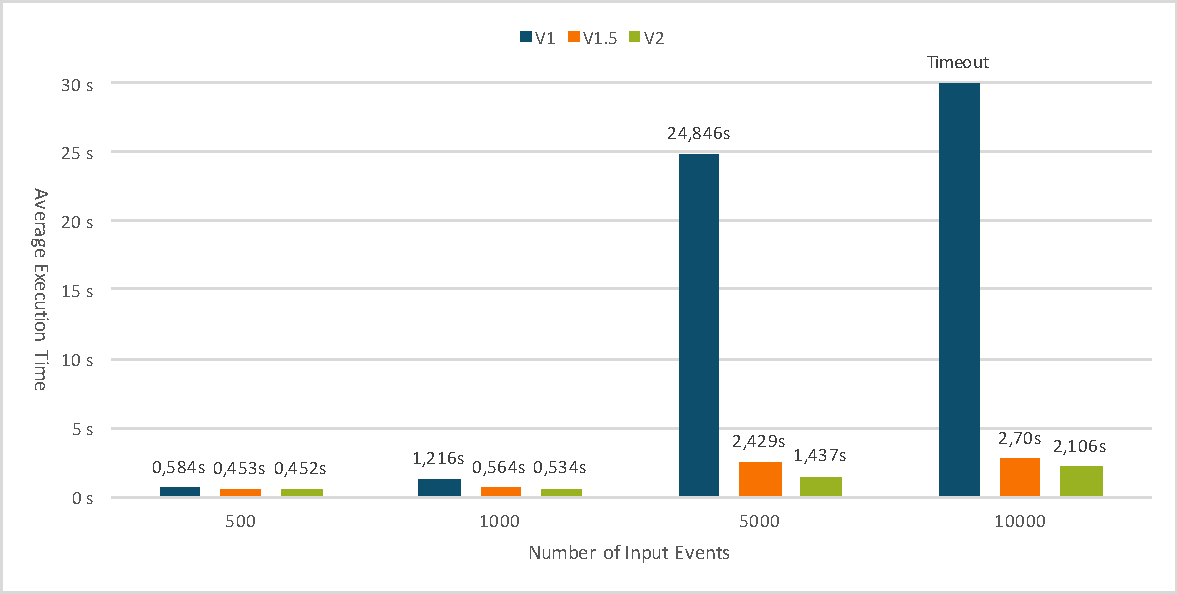
\includegraphics[width=\textwidth]{gfx/runtime_num_events_benchmark}
  \caption[Average execution time of the different implementations when fed with different amounts of input events.]{Average execution time of the different implementations when fed with different amounts of input events. V1 refers to the old approach, V1.5 to the adapted old approach and V2 to the new approach. V1 has no data for 10\,000 events since the enormous \gls{ram} usage constantly lead to timeouts.}
\label{fig:chap_eval:runtime_num_events}
\end{figure}

The number of events also increase memory usage, espacially in the first implementation approach.
The second benchmark therefore tests the \gls{ram} usage of the different approaches under different number of input events.
\Cref{fig:chap_eval:runtime_ram_usage} illustrates the \gls{ram} usage of the different approaches.
The complete data can be found in \cref{table:tessla_server_v1_events_ram_usage_data,table:tessla_server_v1_5_events_ram_usage_data,table:tessla_server_v2_events_ram_usage_data}.

\begin{figure}[!htb]
  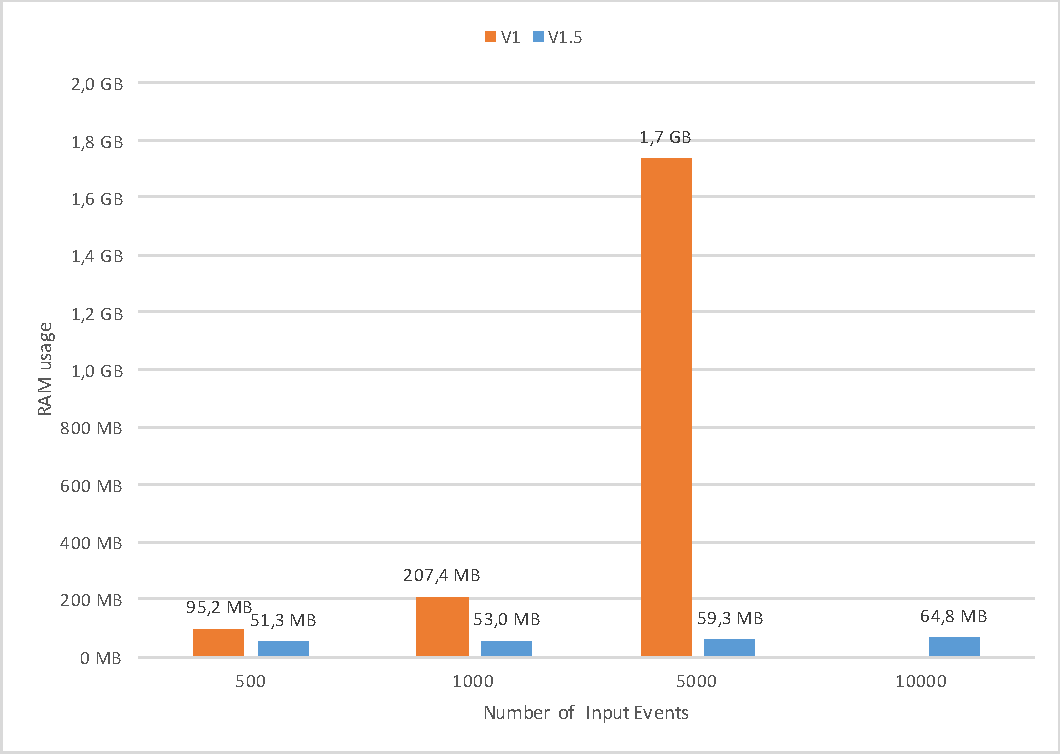
\includegraphics[width=\textwidth]{gfx/runtime_ram_usage_benchmark}
  \caption[\gls{ram} usage of the different versions of the runtime]{\gls{ram} usage of the different versions of the runtime in regard to input events. V1 refers to the old approach, V1.5 to the adapted old approach and V2 to the new approach. V1 has no data for 10\,000 events since the enormous \gls{ram} usage constantly lead to timeouts.}
\label{fig:chap_eval:runtime_ram_usage}
\end{figure}

\subsection{Number of Nodes}

As a last metric the performance of the runtime is evaluated over specifications with different amount of nodes.
Therefore the specification from \cref{listing:runtime_parallel_spec_8} was modified to include higher number of nodes by appending more nodes computing the absolute.
All benchmarks in this section were performed on a processor with 4 cores at 2.4GHz speed and 8GB of \gls{ram}.
\Cref{fig:chap_eval:runtime_num_nodes} visualizes the performance, the complete data can be found in \cref{table:tessla_server_v1_num_nodes,table:tessla_server_v1_5_num_nodes,table:tessla_server_v2_num_nodes}.

\begin{figure}
  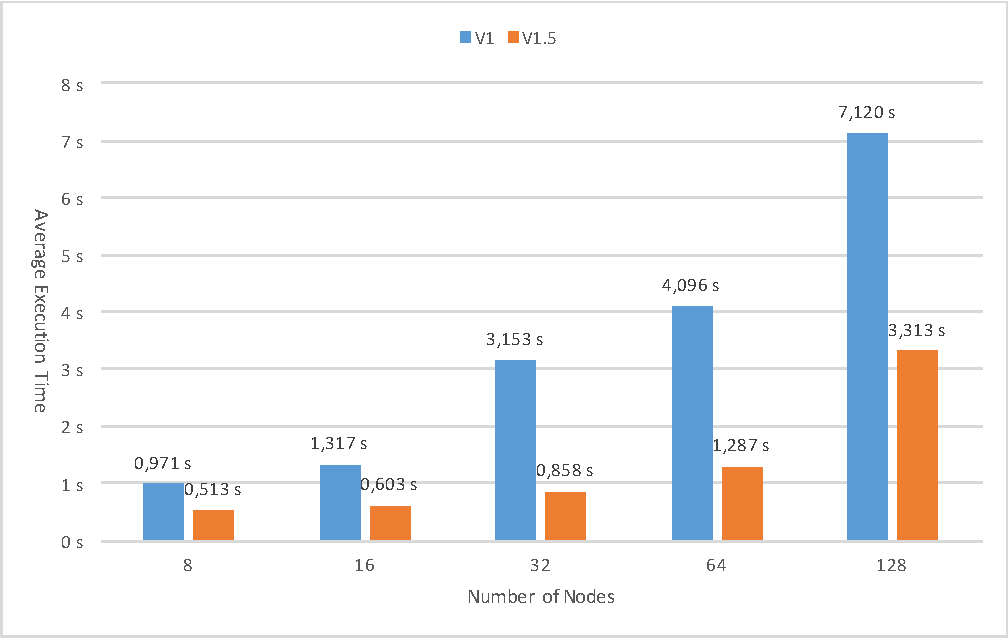
\includegraphics[width=\textwidth]{gfx/runtime_num_nodes_benchmark}
  \caption[Average execution time of the runtime over specifications with different amount of nodes.]{Average execution time of the runtime over specifications with different amount of nodes. All specifications did count the number of function calls and stopped when it reached 1\,000. V1 refers to the old approach, V1.5 to the adapted old approach and V2 to the new approach.}
\label{fig:chap_eval:runtime_num_nodes}
\end{figure}

While there is no real world data of the size of typical \gls{tessla} specifications, 128 nodes seems to be a rational upper bound.
As the data shows the runtime scales nicely with big specification, the data even suggests a somewhat logarithmic increase of the execution time in regard to node count.


\section{Instrumentation Benchmarks}
\label{sec:evaluation:instrumentation_benchmarks}

After the evaluation of the runtime itself it remains to evaluate the C instrumentation program.
Note that the instrumentation is mostly a proof of concept and its main purpose for now was to generate test data for the runtime.
But it seems feasible that it can be optimized and extended to become a general purpose trace collection tool, therefore some benchmarks were performed.

For reliable trace collection of software the performance impact of the instrumentation is important.
To measure this a trivial C program was exercised with and without instrumentation.
The program increments each integer from 0 to 100\,000\,000 by one and, if the incremented number is divisible by a given parameter \(c\), adds it to an intermediate result.
Note that the program  can and will perform some integer overflows.
The code is shown in \cref{listing:instrument_benchmark_code}.

\begin{figure}
\lstinputlisting[language=c, label=listing:instrument_benchmark_code, caption=Example C program for benchmark purposes]{content/code/instrument_benchmark.c}
\end{figure}

The code is then instrumented to log each call of the \lstinline{add} method.
For each benchmark the compiled program was run 50 times.
All benchmarks in this section were performed on an Intel Core i5 with four cores at a clock speed of 2.4GHz and 8GB of Ram.

\subsection{Performance Comparison with non Instrumented Code and Compiler Optimizations}
\label{sec:evaluation:instrumentation_benchmark:instr_vs_non_inst}

One interesting metric is the intrusiveness of the instrumentation, describing how an instrumented program performs in contrast to the same program without the added instrumentation.
For this the parameter \(c\) of the example program is set to 100, so that around 1\% of all function calls are instrumented.

One thing that can be recognized is that the impact of instrumentation is not predictable when using compiler optimizations.
Aggressive compiler optimizations can remove function calls or inline values if the optimization doesn't change the program behaviour.
When instrumentation calls are added no such optimization can happen, since otherwise the behaviour of the program would be altered, namely the logging would be removed when the function calls are removed.

Therefore we compare the instrumented and non-instrumented code for all optimization levels.
The comparison can be seen in \cref{fig:chap_eval:instrument_benchmark_results}.
The complete data can be found in \cref{table:non_instrumented_optimizations_benchmark,table:instrumented_optimizations_benchmark}.

\begin{figure}
  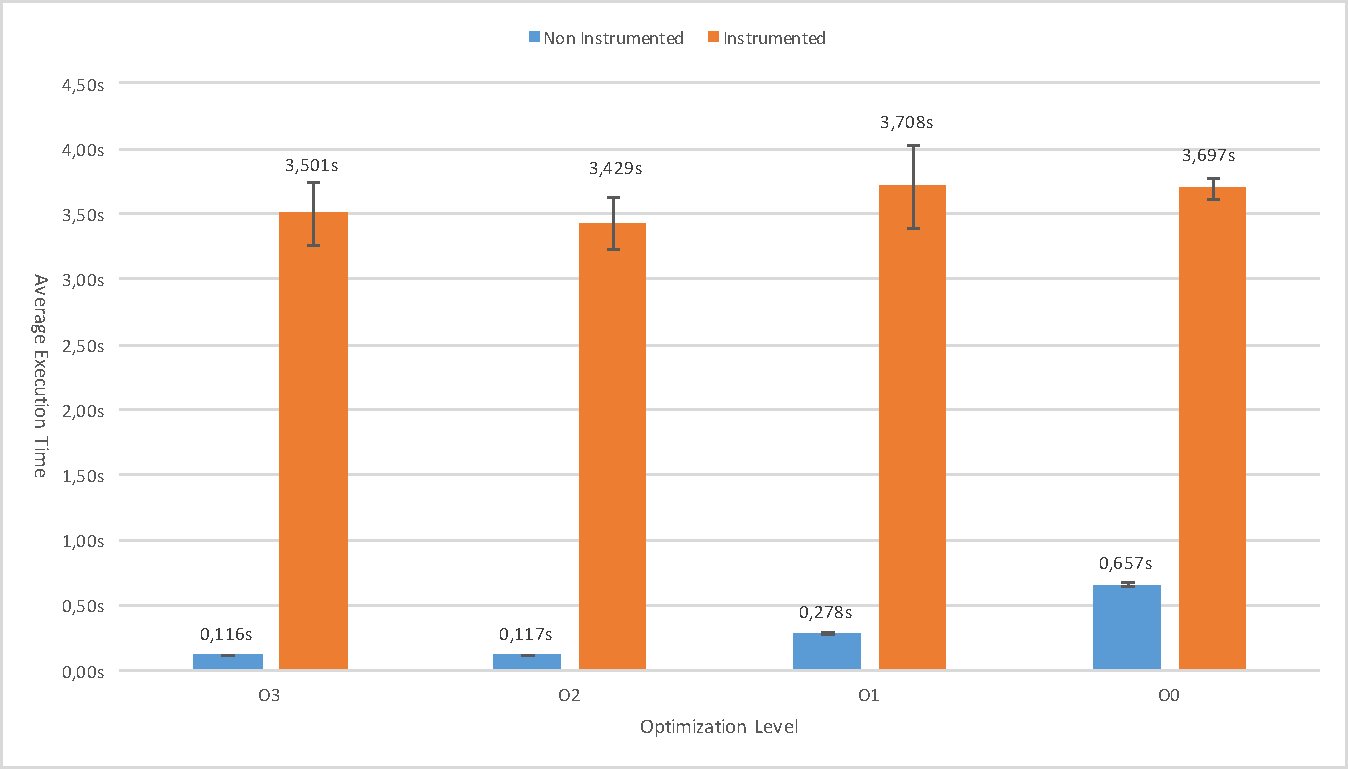
\includegraphics[width=\textwidth]{gfx/instrumentation_time_benchmark}
  \caption{Performance Comparision of an example C program with and without instrumentation.}
\label{fig:chap_eval:instrument_benchmark_results}
\end{figure}

The choice to instrument around 1\% of the function calls was made arbitrary after some experimentation showed that a higher amount leads to huge performance impacts as shown in \cref{sec:evaluation:instrumentation_benchmark:instr_amount}.
Intuitively it sounds reasonable that in a real life example only a small subset of the function calls are interesting for trace generation, since \gls{tessla} specifications should be used to monitor only critical parts of a system.

\subsection{Performance Impact in Regard to Instrumentation Percentage}
\label{sec:evaluation:instrumentation_benchmark:instr_amount}

To further investigate the impact of instrumentation we will look at the performance impact with respect to the percentage of function calls that are instrumented.
Therefore the variable \(c\) of the program is changed, which leads to different amount of calls to the instrumented function.
For all values the program was compiled with the maximal optimization setting.
In \cref{fig:chap_eval:instrument_benchmark_amount_results} the results of changing the parameter can be seen.
The complete dataset can be found in \cref{table:instrumented_amount_benchmark}.

\begin{figure}
  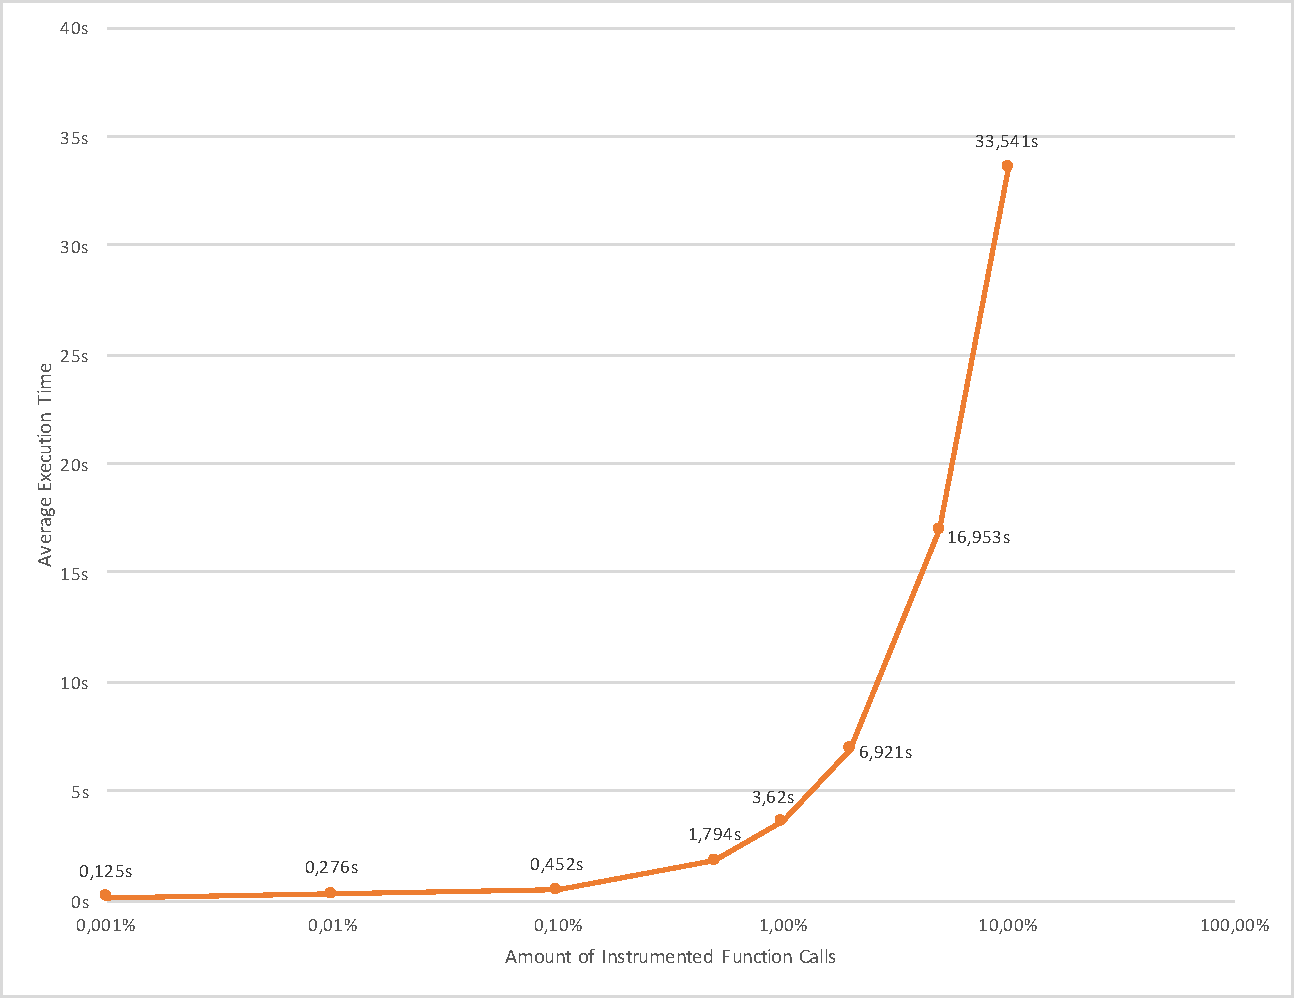
\includegraphics[width=\textwidth]{gfx/instrumentation_amount_benchmark}
  \caption{Execution time of a program with different amount of calls to an instrumented function}
\label{fig:chap_eval:instrument_benchmark_amount_results}
\end{figure}

Note that the \(x\)-axis is logarithmic.
As expected the performance impact scales directly with the amount of calls to the instrumented function.
At some point no more speed up will happen, since no calls to the instrumented functions will be made.

\section{Practical Examples}
\label{sec:evaluation:runtime_examples}

Additionally to the theoretic benchmarks it was also important to evaluate the runtime against some more practical examples and test a bigger amount of node types.
While the specifications for the benchmarks from the previous section did use some node types and showed that these types perform the correct computations (else the benchmarks wouldn't have worked), they only used a subset of all available types.
Thus the following examples concentrate on a wider range of different nodes.

To do so traces from real world examples were collected, either with the developed instrumentation pass or by adjusting existing logs to fit the needs of \gls{tessla}.
The programs or traces were then modified to deliberately include errors to test if appropriate \gls{tessla} specifications will find them when evaluated in the runtime.

% \subsection{Ringbuffer Examples}

As the main source for test trace data a ringbuffer, implemented in C, was modified by the instrumentation to log specific events.
The code of the ringbuffer can be found in \cref{listing:ringbuffer}.
Events that are logged are of two types: calls to the \lstinline{process} function and changes of the \lstinline{write_ptr} variable.
The generated traces can be used for a variety of specifications, e.g.: performance tests, race conditions or wrong initilizations.

Following specification were tested over the traces:

\begin{itemize}
  \item Data is only processed, when it is available, meaning that at each point of the trace the amount of changes of \lstinline{write_ptr} is bigger than the number of calls to \lstinline{process}.
  \item The given buffer size of five is never exceeded, meaning the difference of the amount of changes of both event types is never bigger than five.
  \item Everytime new data is added, there is a call to process in the next milisecond.
\end{itemize}

The specifications were intentionally chosen and written in such a way, that they use a big amount of different nodes.
For each of these specification the traces were deliberately altered to violate them.
Evaluation of the specifications over the traces with TesslaServer always led to the correct conclusions.
